\documentclass{article}
% Revised preamble for the jmlr conference template

\usepackage{hyperref}       % hyperlinks
\usepackage{url}            % URL typesetting
\usepackage{booktabs}       % professional-quality tables
\usepackage{amsmath, amsfonts, amssymb} % math packages
\usepackage{mathtools}      % extended math tools
\usepackage{nicefrac}       % compact fractions
\usepackage{microtype}      % microtypography
\usepackage{cleveref}       % intelligent cross-referencing
\usepackage{graphicx}       % graphics
\usepackage{natbib}         % bibliography support
\usepackage{doi}            % DOI formatting
\usepackage{subfiles}       % subfile support
\usepackage{listings}       % source code listings
\usepackage[normalem]{ulem} % underline/strikeout (remove before final submission)
\usepackage[]{todonotes}    % inline todo notes (optional)
\usepackage{orcidlink}
\usepackage{xparse}

% TikZ for diagrams (if needed)
\usepackage{tikz}
\usetikzlibrary{shapes,arrows,calc,positioning,automata,decorations.pathreplacing,quotes}
\usetikzlibrary{bayesnet}

% Custom commands and notation
\newcommand{\Ex}{\mathbb{E}}
\newcommand{\var}{\operatorname{Var}}
\newcommand{\cov}{\operatorname{Cov}}
\newcommand{\corr}{\operatorname{Corr}}
\newcommand{\argmin}{\operatorname{arg\,min}}
\newcommand{\argmax}{\operatorname{arg\,max}}
\newcommand{\diag}{\operatorname{diag}}
\newcommand{\vecop}{\operatorname{vec}}
\newcommand{\dd}{\mathrm{d}}
\newcommand{\pd}{\mathrm{d}}
\newcommand{\bb}[1]{\mathbb{#1}}
\newcommand{\vv}[1]{\boldsymbol{#1}}
\newcommand{\mm}[1]{\mathrm{#1}}
\newcommand{\mmmean}[1]{\bar{\mathrm{#1}}}
\newcommand{\mmdev}[1]{\breve{\mathrm{#1}}}
\newcommand{\rv}[1]{\mathsf{#1}}
\newcommand{\vrv}[1]{\vv{\rv{#1}}}
\newcommand{\dist}[1]{\mathcal{#1}}
% \newcommand{\set}[1]{\mathcal{#1}}
\newcommand{\op}[1]{\mathcal{#1}}
\newcommand{\proj}{\mm{P}}
\newcommand{\disteq}{\stackrel{\mathrm{d}}{=}}
\newcommand{\Normal}{\mathcal{N}}
\newcommand{\approxdisteq}{\stackrel{\mathrm{d}}{\approx}}
\newcommand{\gvn}{\mid}
\renewcommand{\Pr}{\mathbb{P}}
\newcommand{\solop}{\mathcal{G}^{\dagger}}
%
% Measure notation commands:

\NewDocumentCommand{\Law}{o}{%
  \mu\IfValueT{#1}{_{#1}}%
}

\NewDocumentCommand{\ELaw}{o}{%
  \widehat{\mu}\IfValueT{#1}{_{#1}}%
}
% Independence symbol
\newcommand\indep{\protect\mathpalette{\protect\independenT}{\perp}}
\def\independenT#1#2{\mathrel{\rlap{$#1#2$}\mkern2mu{#1#2}}}

\newcommand{\one}{\mathbbold{1}}

% \theoremstyle{plain}
% \newtheorem{theorem}{Theorem}[section]
% \newtheorem{lemma}[theorem]{Lemma}
% \newtheorem{definition}[theorem]{Definition}
% \newtheorem{proposition}[theorem]{Proposition}

% Recommended, but optional, packages for figures and better typesetting:
\usepackage{microtype}
\usepackage{graphicx}
%\usepackage{subfigure}
\usepackage{booktabs} % for professional tables

% hyperref makes hyperlinks in the resulting PDF.
% If your build breaks (sometimes temporarily if a hyperlink spans a page)
% please comment out the following usepackage line and replace
% \usepackage{icml2023} with \usepackage[nohyperref]{icml2023} above.
\usepackage{hyperref}


% Attempt to make hyperref and algorithmic work together better:
\newcommand{\theHalgorithm}{\arabic{algorithm}}

% Use the following line for the initial blind version submitted for review:
\usepackage{icml2023}

% If accepted, instead use the following line for the camera-ready submission:
% \usepackage[accepted]{icml2023}

% For theorems and such
\usepackage{amsmath}
\usepackage{amssymb}
\usepackage{mathtools}
\usepackage{amsthm}

% if you use cleveref..
%\usepackage[capitalize,noabbrev]{cleveref}

%%%%%%%%%%%%%%%%%%%%%%%%%%%%%%%%
% THEOREMS
%%%%%%%%%%%%%%%%%%%%%%%%%%%%%%%%
\theoremstyle{plain}
\newtheorem{theorem}{Theorem}[section]
\newtheorem{proposition}[theorem]{Proposition}
\newtheorem{lemma}[theorem]{Lemma}
\newtheorem{corollary}[theorem]{Corollary}
\theoremstyle{definition}
\newtheorem{definition}[theorem]{Definition}
\newtheorem{assumption}[theorem]{Assumption}
\theoremstyle{remark}
\newtheorem{remark}[theorem]{Remark}

% Todonotes is useful during development; simply uncomment the next line
%    and comment out the line below the next line to turn off comments
%\usepackage[disable,textsize=tiny]{todonotes}
%\usepackage[textsize=tiny]{todonotes}


% The \icmltitle you define below is probably too long as a header.
% Therefore, a short form for the running title is supplied here:



\icmltitlerunning{The Ensemble Kalman Update as Matheron update}

% Here you can change the date presented in the paper title
%\date{September 9, 1985}
% Or remove it
%\date{}

%\author{ \href{https://orcid.org/0000-0001-6077-2684}{
\includegraphics[scale=0.06]{orcid.pdf}\hspace{1mm}Dan B MacKinlay}%\thanks{Use footnote for providing further
		%information about author (webpage, alternative
		%address)---\emph{not} for acknowledging funding agencies.}
%  \\\
%	CSIRO's Data61 \\
%	\texttt{Dan.MacKinlay@data61.csiro.au} \\
%	%% examples of more authors
%	\And
%	Dan Pagendam \\
%		CSIRO's Data61 \\
%	\AND
%	Russell Tsuchida \\
%	CSIRO's Data61 \\
%	\And
%	Petra Kuhnert \\
%	CSIRO's Data61 \\
%	\And
%	   Sreekanth Janardhanan \\
%	CSIRO \\
%}


\begin{document}

\twocolumn[
\icmltitle{The Ensemble Kalman Update is an empirical Matheron update}

% It is OKAY to include author information, even for blind
% submissions: the style file will automatically remove it for you
% unless you've provided the [accepted] option to the icml2023
% package.

% List of affiliations: The first argument should be a (short)
% identifier you will use later to specify author affiliations
% Academic affiliations should list Department, University, City, Region, Country
% Industry affiliations should list Company, City, Region, Country

% You can specify symbols, otherwise they are numbered in order.
% Ideally, you should not use this facility. Affiliations will be numbered
% in order of appearance and this is the preferred way.
\icmlsetsymbol{equal}{*}



\begin{icmlauthorlist}
\icmlauthor{Firstname1 Lastname1}{equal,yyy}
\icmlauthor{Firstname2 Lastname2}{equal,yyy,comp}
\icmlauthor{Firstname3 Lastname3}{comp}
\icmlauthor{Firstname4 Lastname4}{sch}
\icmlauthor{Firstname5 Lastname5}{yyy}
\icmlauthor{Firstname6 Lastname6}{sch,yyy,comp}
\icmlauthor{Firstname7 Lastname7}{comp}
%\icmlauthor{}{sch}
\icmlauthor{Firstname8 Lastname8}{sch}
\icmlauthor{Firstname8 Lastname8}{yyy,comp}
%\icmlauthor{}{sch}
%\icmlauthor{}{sch}
\end{icmlauthorlist}

\icmlaffiliation{yyy}{Department of XXX, University of YYY, Location, Country}
\icmlaffiliation{comp}{Company Name, Location, Country}
\icmlaffiliation{sch}{School of ZZZ, Institute of WWW, Location, Country}

\icmlcorrespondingauthor{Firstname1 Lastname1}{first1.last1@xxx.edu}
\icmlcorrespondingauthor{Firstname2 Lastname2}{first2.last2@www.uk}

% You may provide any keywords that you
% find helpful for describing your paper; these are used to populate
% the "keywords" metadata in the PDF but will not be shown in the document
\icmlkeywords{likelihood free, ensemble, Gaussian Process, inverse modelling, physics}

\vskip 0.3in
]

% this must go after the closing bracket ] following \twocolumn[ ...

% This command actually creates the footnote in the first column
% listing the affiliations and the copyright notice.
% The command takes one argument, which is text to display at the start of the footnote.
% The \icmlEqualContribution command is standard text for equal contribution.
% Remove it (just {}) if you do not need this facility.

\printAffiliationsAndNotice{}  % leave blank if no need to mention equal contribution
%\printAffiliationsAndNotice{\icmlEqualContribution} % otherwise use the standard text.

\begin{abstract}
    A popular means of

    The cost of the resulting algorithm scales linearly with the dimension of the estimands and  does not require the calculation or storage of large covariance matrices.
    %Nor does it require artificial evolution dynamics to be applied to static latent parameters.
    We do not require exact likelihood evaluations of the prior or posterior samples.
    However, we do require the ability to simulate from the prior, and sufficient regularity of the forward operator.
    Our method achieves orders-of-magnitude speed-up over a classical physical model inversion approach for high-dimensional models, while maintaining acceptable accuracy. This increases the dimensionality of the estimand at which inference is feasible, without resorting to dimension reduction methods.
    % \russ{Abstracts should be 4-6 sentences and a single paragraph}
    \footnote{\textcolor{blue}{Link to publically available code to be provided upon acceptance. Reviewers, see attached .zip.}}
\end{abstract}

\section{Introduction}
This paper introduces a method for inversion of models of dynamical systems whose state and static parameters are both very high-dimensional and highly correlated, but which may be modelled by a physic simulator.
Problems of this sort arise in geophysics, hydrology, and medical imaging, and are central to many problems in machine learning.
In fact, inferring any hidden cause through its influence on some dynamical behaviour may be understood as a problem of this type.
Traditionally, the methods to solve inverse problems have been statistical \cite{TarantolaInverse2005} and have often relied on strategies like model emulation / surrogate modelling and dimension reduction to make these feasible in applied settings.

 We propose the MaTHeron Ensemble inversion approach (\meth{}), which efficiently utilises a (possibly black-box) forward operator to sample from a posterior distribution over unobserved  static parameters.
\meth{} advances our capability to handle such models, by treating the observations as an  approximation to Gaussian variates utilising the the ensemble methods of the data assimilation community~\cite{EvensenData2009}.
Gaussian variates may be updated, sample-wise, using the Matheron update~\cite{DoucetNote2010,WilsonEfficiently2020}, without the need to calculate covariances explicitly.
The method is general enough to be applicable to any dynamic model that is well-approximated by assuming linearity in expectation, scales to very large systems, and requires few assumptions.
% The prior distributions may be supplied by any model from which we can sample, and are not required to, for example, possess stationary or homogenaeity.

The method is structurally similar to the Ensemble Kalman filter, in that all updates between random variates are conducted via ensembles of samples rather than explicit densities.
However, \meth{} exploits the closed form Matheron updates for static parameters rather than states. This generates closed-form ensemble update rules which are capable of assimilating multiple observations without ever constructing the prior covariance matrix, and thus scales to very high dimensions.

\section{Preliminaries}

\subsection{Notation}
We adopt the following notation. A variable displayed like $\statest_{t}$ represents the realisation of a function (e.g. a spatial field) indexed at time $t$; the variable displayed sans-serif $\state_{t}$ represents a random variable used to model (statistically) $\statest_{t}$.
%capital letters in calligraphic font, such as $\statesp$, represent the space of a variable like $\statest_{t}$;
% bold, lowercase letters like ${\state}_{t}$ denote finite dimensional vectors
%(e.g. the pointwise evaluations on $\state_t$);
%matrices are represented by capital letters such as $K$, but this is not exclusive;
For simplicity, we assume that all random variables have a probability distribution that is absolutely continuous with respect to Lebesgue measure.
That is, all random variables admit a probability density function, although this density function is not evaluated in the computations involved in our technique.
% Our methods similarly apply to probability distributions that do not admit a probability density function, although their use may not necessarily be appropriate.
Following conventional notation, we write $p(\cdot)$ for the probability density of a random variable, and $p(\cdot \mid \cdot)$ for conditional densities, where the meaning of $p$ is clear from context.
We notate that a random variable $\state_t$ follows a distribution with probability density $p$ by $\state_t \sim p(\statest_t)$.

\subsection{Related work}

Model inversion has a long history of methodological development in the geophysical sciences, where problems often involve high-dimensional parameter spaces and complex physical models.  Popular approaches for inversion in these fields include GLUE \cite{Beven2014}, PEST \cite{Doherty2010}, DREAM \cite{Vrugt2011} and MCMC algorithms \cite{Oh2001}.

In the broader scientific community, model inversion has often utilised standard Bayesian statistical approaches \cite{StuartInverse2010,DashtiBayesian2015,TarantolaInverse2005}.  For high-dimensional, computationally expensive simulators, model inversion has often involved the use of model emulation (surrogate modelling) \cite{Hooten2011FirstOrder, GramacyLocal2015, Gopalan2021HOSVD, ColeLocallyInduced2021} and/or dimension reduction methods \cite{Higdon2008SVDEmulator, SiadeSnapshot2010, Grana2019}, both of which introduce additional uncertainties into the inferential process.

More recently, machine learning methods for model inversion have become an active area of research.  For example, the use of Physics-Informed Neural Networks (PINNs) \cite{HePhysicsinformed2020,YangPhysicsInformed2020,ZhangLearning2020}; stochastic inversion via adversarial learning~\cite{XuAdversarial2019,BaoNumerical2020,ChuLearning2021}; operator inversion with diffusion models~\cite{SongSolving2022,JalalRobust2021};
neural operator inversion with graph neural networks~\cite{LiNeural2020};
Bayesian neural operators with last-layer Laplace approximations~\cite{MagnaniApproximate2022}; neural linear models with functional GP priors \cite{WatsonNeural2020}.

Amongst these machine learning methods, Gaussian processes have a prominent place.  For inverse problems with large numbers of observations and/or with high-dimensional data, it is common to resort to sparse GP approximations for computational feasibility.  Methods include the use of inducing points \cite{Bauer2016} and Vecchia approximations \cite{Katzfuss2020}, both of which reduce the computational complexity by introducing a simpler approximation to the likelihood function.

In contrast, this work is positioned in the larger field of ``likelihood-free'' methods (e.g.~\citet{CranmerFrontier2020}) in that we endeavour to conduct inference for complex physical models without evaluating explicitly the likelihoods for the observations.  The approach makes use of Gaussian processes, but avoids making approximations of the process by working with an ensemble of samples instead.

\subsection{Gaussian updates}
The multivariate Gaussian distribution enjoys a host of mathematically convenient properties.
One of the most widely exploited properties is the fact that jointly Gaussian random variables are closed under conditioning on values of coordinates of the random variables.
We will leverage this fact in two forms.
The first form, invoked in \S~\ref{sec:error_prop}, describes the conditioning operation in terms of probability densities.
The second form, invoked in \S~\ref{sec:EnsembleInversion} describes the conditioning operation in terms of random vectors.

\paragraph{Distributional conditioning}
We repeatedly exploit the following well-known property of multivariate Gaussians.
Jointly Gaussian variates,
\begin{align*}
    \begin{bmatrix}\vrv{y}\\ \vrv{w}
\end{bmatrix}\sim\mathcal{N}\left(\begin{bmatrix}
    \vv{m}_{\vrv{y}}\\ \vv{m}_{\vrv{w}}
\end{bmatrix},\begin{bmatrix}
    \mm{K}_{\vrv{y}\vrv{y}} & \mm{K}_{\vrv{y}\vrv{w}} \\
    \mm{K}_{\vrv{w}\vrv{y}} & \mm{K}_{\vrv{w}\vrv{w}}
\end{bmatrix}\right) \numberthis \label{eq:jointly_gaussian}
\end{align*}
have a data-conditional update, namely,
\begin{align*}
p(\vv{y}\gvn &\vrv{w}{=}\vv{w})=\dist{N}\left(
        \hat{\vv{m}},
        \hat{\mm{K}}
\right), \quad \text{where} \numberthis\label{eq:cond-joint-normal} \\
\hat{\vv{m}}
    &=\vv{m}_{\vrv{y}}
        +\mm{K}_{\vrv{y}\vrv{w}} \mm{K}_{\vrv{w}\vrv{w}}^{-1}(\vv{w}- \vv{m}_{\vrv{w}}), \quad \text{and} \numberthis \label{eq:gaussian-cond-mean}\\
\hat{\mm{K}}
    &=\mm{K}_{\vrv{y}\vrv{y}}
        -\mm{K}_{\vrv{y}\vrv{w}} \mm{K}_{\vrv{w}\vrv{w}}^{-1}\mm{K}_{\vrv{w}\vrv{y}}.\numberthis\label{eq:gaussian-cond-var}
\end{align*}

\paragraph{Pathwise conditioning via Matheron updates} In this work we leverage a technique that we call the \emph{Matheron update}, which is a means of perturbing samples from jointly Gaussian random variate into samples conditional on a practical observation by additive updates.
Whereas~\eqref{eq:cond-joint-normal},~\eqref{eq:gaussian-cond-mean} and~\eqref{eq:gaussian-cond-var} describe the conditioning operation in terms of moments, the Matheron update describes the conditioning operation in terms of random variables.
Let $\vrv{y}$ and $\vrv{w}$ be jointly Gaussian according to~\eqref{eq:jointly_gaussian}.
Then samples from the conditional distribution with conditional density $p(\vv{y} \mid \vrv{w} = \vv{w})$ satisfy the following relation to samples from the unconditional joint density
\begin{align*}
    \vrv{y} \gvn (\vrv{w}{=}\vv{w}) \stackrel{d}{=} \vrv{y}
        +\mm{K}_{\vrv{y}\vrv{w}} \mm{K}_{\vrv{w}\vrv{w}}^{-1}(\vrv{w} - \vv{w}). \numberthis \label{eq:matheron_rule_1}
\end{align*}
\iffalse
Or in density notation,
\begin{align*}
&(y^{(0)},w^{(0)})\sim p(\vv{y},w)\\
&\Rightarrow y^{(0)} +\mm{K}_{\vrv{y}\vrv{w}} \mm{K}_{\vrv{w}\vrv{w}}^{-1}(w - w^{(0)}) \sim p(\vv{y}\gvn \vrv{w}{=}w)
\end{align*}
 where we use \(\sim\) to mean ``is sampled from'' rather than ``is distributed according to``.
\fi
This identity can be verified by taking the expectation and covariance of both sides of~\eqref{eq:matheron_rule_1} and noting that linear combinations of Gaussian random variables are Gaussian, as presented in~\citet[Theorem 1]{WilsonEfficiently2020}.

In machine learning this identity is known as the Matheron or \emph{pathwise} update
(e.g.~\citet{DoucetNote2010,RitterScalable2018,WilsonPathwise2021}). The Matheron update gives us a means to move from random samples from a given distribution, to random samples from that distribution conditioned upon some observation. %For an in-depth explanation, see Appendix~\ref{app:matheron}.
 % \russ{Is this the same notation issue again? Don't we want the conditional given all the past states, not just the last two?}
Applications in the geoscience and data assimilation literature uses distinct terminology, e.g. \emph{conditional simulation update}~\citep{KatzfussUnderstanding2016}, or \emph{ensemble perturbation}~\citep{EvensenData2009}.
In the current work, we connect the use of the update rule in these distinct fields.

\section{Problem setting}
\paragraph{Forward model}
Let  $\state_t\in \statesp \subset \mathbb{R}^{D_{\state}}$ for each $t=0,1,2,\ldots,T$ be a sequence of states, with $\state_0=\statest_0$ known.
The state dynamics arise from recursive application of a \emph{forward operator} \(\op{P}:\statesp\times  \forcingsp \to \statesp\) whose action is known conditional on an unknown time-invariant parameter, \(\forcing\in\forcingsp\subset \mathbb{R}^{D_{\forcing}}\), such that
\begin{align*}
    \state_{t}=\op{P}(\state_{\tm}, \forcing),\quad t=1, 2, \cdots, T.\numberthis\label{eq:ts-sem}
\end{align*}
Formally, we allow \(\op{P}\) to be stochastic, which we can make explicit by adding an unobserved white noise \(\vrv{\nu}_{t}\) to the arguments of $\op{P}$.
Equivalently, we may express a likelihood over current states given previous states and parameter. That is, there exists some nonnegative and appropriately normalised $f$ such that for each $t = 1,\ldots,T$,
\begin{equation}
\begin{aligned}
    \state_{t}&=\op{P}(\state_{\tm}, \forcing, \vrv{\nu}_{\tm}),  \\
    \iff p(\statest_t \gvn \state_{t-1}, \forcing) &= f(\statest_t; \state_{t-1}, \forcing).
\end{aligned}
\label{eq:ts-sem-stoch}
\end{equation}

The techniques that are available and suitable for inference depend on the degree to which the forward model is known.
We distinguish between two degrees of such knowledge.
If we may evaluate $f$ and its derivatives at any point,
or we can evaluate $\op{P}$ and its derivatives at any point, we call the forward model a \emph{white-box} model.
If we can evaluate only $\op{P}$, we call the forward model a \emph{black-box} model.
Note that we assume the state dynamics has the Markov property, so that the likelihood factors as
\begin{align*}
    p(\statest_1, \ldots, \statest_T \gvn \forcing ) &= \prod_{t=1}^T p(\statest_t \gvn \state_{t-1}, \forcing) p(\forcing). \numberthis \label{eq:likelihood}
\end{align*}


\paragraph{Discrete bases} In the physical problems that motivate our approach, vectors possess an interpretation as a finite dimensional representation of a physical system of interest, as the coefficients of a projection of the system onto an orthogonal basis.
For example we could have \(\state_{t}\) represent instantaneous, discretised density and velocity field of a fluid distributed over some spatial domain, \(\op{P}\) the discretised forward predictor of a noisy fluid simulation, and the parameter $\forcing$ an inhomogenous forcing term arising from an external driver applied to the system.
Such a finite representation is consistent with the way in which state dynamics are typically manipulated in machine learning settings (such as~\S 2.2 of~\citet{RasmussenGaussian2006}), where inference over finitely many evaluations is of primary concern.
Although the forward operator and vector space are both assumed to arise from some discretisation of a continuous-time, continuous-space system, we do not concern ourselves with the details of discretisation here. Instead, we assume that the discretisation error may be made negligible if the problem is discretised to a ``fine-enough basis'' e.g.~\cite{LassasDiscretizationinvariant2009}, for which it is necessary that we can handle high-dimensional state vectors.
In the examples here the bases are finite-element bases of top hat functions (Appendix~\ref{app:basis-functions}).

\paragraph{Bayesian inference} A Bayesian probabilistic model represents the quantities of interest with random variables by assigning some probability measure over the state space.
We represent our \emph{prior} belief (before observing any data) over plausible values that the parameter $\forcing$ can take using probability.
An appropriate choice of prior measure regularises our inference towards some plausible region of solution space.
We place a prior probability density function over $\forcing$ and write $p(\forcingst)$ for the evaluation of such a density.
For concreteness, we take the prior $p(\forcingst)$ to be a multivariate Gaussian, however the methods we discuss may utilise more general priors.
That is, the parameter prior satisfies
\begin{align*}
\forcing \sim \dist{N}(m_0,\mm{K}_0),
\end{align*}
where $\mm{K}_0 \in \mathbb{S}^{D_{\forcing}}_+$ is a PSD covariance matrix and $m_0 \in \mathbb{R}^{D_{\forcing}}$ is a mean vector.

Our goal is to sample values of the parameter $\forcing$ given the observations  \(\set{D}_T=\{\state_1=\statest_1, \cdots, \state_T=\statest_T\}\). That is, we seek to approximately compute, sample from, or otherwise describe (some property of) the \emph{posterior}
% We approach this in a probabilistic setting where both estimands and observations may be random variables.the posterior
\begin{align*}
    p\big( \forcingst \gvn \mathcal{D}_T \big) =  \frac{p(\forcingst) p(\mathcal{D}_T \gvn \forcingst)}{p(\mathcal{D}_T)},\numberthis \label{eq:bayes_rule}
\end{align*}
where the likelihood $p(\mathcal{D} \gvn \forcingst)$ admits a factorisation via~\eqref{eq:likelihood}.



For compactness we  define \(\forcing_{t}:=\forcing\gvn (\state_{0}{=}\statest_{0},\dots,\state_{t}{=}\statest_{t})\), and note that
% \russ{I can't see this factorisation --- does it rely on a kind of Bayes' rule?}
\begin{align*}
% \left(\forcing\gvn \state_{0}{=}\statest_{0},\dots,\state_{t}{=}\statest_{t}\right)
% &= \left(\left(\forcing\gvn \state_{0}{=}\statest_{0},\dots,\state_{\tm}{=}\statest_{\tm}\right) \gvn\state_{\tm}{=}\statest_{\tm},\state_{t}{=}\statest_{t}\right)\\
p(\forcing_{t})
&= p\left(\forcing_{\tm}\gvn
\state_{\tm}{=}\statest_{\tm},
\state_{t}{=}\statest_{t}
\right).\numberthis\label{eq:filtering}
\end{align*}
For a derivation of this rule, see Appendix~\ref{app:conditioning-dag}.

The dynamical systems we study are of the following form:
At each time \(t\), the system state is some spatial field
\(\op{P}:\statesp\times  \forcingsp \to \statesp\) that maps a temporally evolving process from forcing space \( \forcingsp\) and state space \(\statesp\) at time $t-1$ to state space \(\statesp\) at time $t$, and where each of \(\statesp,\forcingsp\) is a (possibly random) vector space.
Recursive application of the forward operator using
\begin{align*}
    \statest_{t}=\op{P}(\statest_{\tm}, \forcingst)
\end{align*}
defines a time series, ${\statest}_{0:T} = (\statest_0, \statest_1, \cdots, \statest_T)$.


If we introduce randomness into this system, for example by allowing forcings, initial conditions to be random, or a random perturbation to the forward operator, then we write this as a random series, $\state_{0:T} = (\state_0, \state_1, \cdots, \state_T)$.

\emph{Inverse problems} in this context are problems of the following sort:
Assume the initial state is some random  \(\state_0\sim \pi\) and unobserved, can we estimate it from a realisation of the time series, \(\state_{1:T} = \statest_{1:T}
\)?
We will assume a  a prior \(\pi\) over \(\state_{0}\) encodes our  beliefs about the qualities of solutions, favouring, e.g. smoothness.

Our method defines a coupled Gaussian Process representation of input and output fields\nb{cite some spatial GP people}, and then exploits the pathwise updates~\cite{WilsonEfficiently2020} to sample from the model posterior.
Finally, ensemble data assimilation~\cite{EvensenData2009,RothEnsemble2017} accumulates updates from multiple timesteps.

\paragraph{Bayesian network and recursive updates} Recursive application of the forward operator
\begin{align*}
\state_{t}
% \gvn \state_{\tm},\forcing
&= \op{P}(\state_{\tm},\forcing ), \quad t=1,\cdots,T,
\numberthis \label{eq:proc_proj_sem_inv}
\end{align*}
given some known initial state \(\state_{0}=\statest_0\), defines a time series of random vectors, $\state_{1:T} := (\state_1^{\top}, \ldots, \state_T^{\top})^{\top}$.

The corresponding Bayesian network, depicted in Figure~\ref{fig:ts_dag}, defines a simple dependence structure between field-valued variates, although \emph{within} a (vector-valued) variate we permit arbitrary dependencies between sites.

\subfile{bayesnet}

Except in a small number of cases, the distribution induced by this definition has no closed form representation.
A notable exception is the case in which Gaussian distributions are perturbed by linear operators, resulting in another Gaussian distribution~(\citealp{RasmussenGaussian2006}~\S~2.2; \citealp{solak2002derivative}; \citealp{ghosal2006posterior}~Theorem~5).
\russ{Broken references?}

We can use the independence structure of the variates to iteratively update posteriors at time $T-1$ into posteriors at time $T$ by conditioning on successive observations, since
\begin{align*}
    &\phantom{{}={}} p(\forcingst \gvn \mathcal{D}_{t}) \\
    &= p(\forcingst \gvn \mathcal{D}_{t-1} ) \frac{ p(\mathcal{D}_t \gvn \mathcal{D}_{t-1}, \forcingst)}{p(\mathcal{D}_t)} \\
    &= p(\forcingst \gvn \mathcal{D}_{t-1} ) \frac{ p(\statest_t \gvn \state_{t-1}, \forcingst)}{p(\mathcal{D}_{t-1})\int p(\statest_t \gvn \state_{t-1}, \forcingst') p(\forcingst') \, d\forcingst'}.
\end{align*}


Unfortunately, computing the posterior even using recursive updates is usually intractable.
The %pushforward measure (i.e.
probability measure of the random variable $\state_t = \op{P}(\state_{t-1}, \forcing)$  can be arbitrarily complicated, and thus the posterior~\eqref{eq:bayes_rule} induced by \eqref{eq:proc_proj_sem_inv} will typically be intractable.
% The normalising constant $p(\mathcal{D}_t)=\int p(\mathcal{D}_t \gvn \forcingst') p(\forcingst') \, d\forcingst'$ is the source of intractability.
Popular approaches for estimating/approximating the posterior distribution in the absence of the normalising constant are to either: (i) use sampling algorithms like Markov Chain Monte Carlo (MCMC) and importance sampling (IS)); or (ii) impose a particular parametric distribution on the posterior (e.g. variational inference and Laplace approximations).
We leverage both in what follows.

\paragraph{Example} For concreteness we use a specific example throughout this paper, illustrated in  Figure~\ref{fig:dynamicalsystem}.
The forward operator $\op{P}$ applies incompressible Navier-Stokes fluid flow forward-propagation equations on a square domain.
The state $\state_t$ of the system is by assumption completely characterised by a discretisation of the problem into a locally-constant \(256\times 256\) lattice of cells, each of which possesses a density (\ref{fig:states}) and two-dimensional velocity (not shown) for an overall state dimension of \(D_{\state}=256\times 256 \times (1+2)\).
The latent parameter $\forcing$, a discretised 2-vector field, is characterised completely by a vector of dimension \(D_{\forcing}=256\times 256 \times 2\).

% \begin{figure*}[h!t]
%      \centering
%     \begin{subfigure}{0.7\textwidth}
%         \centering
%         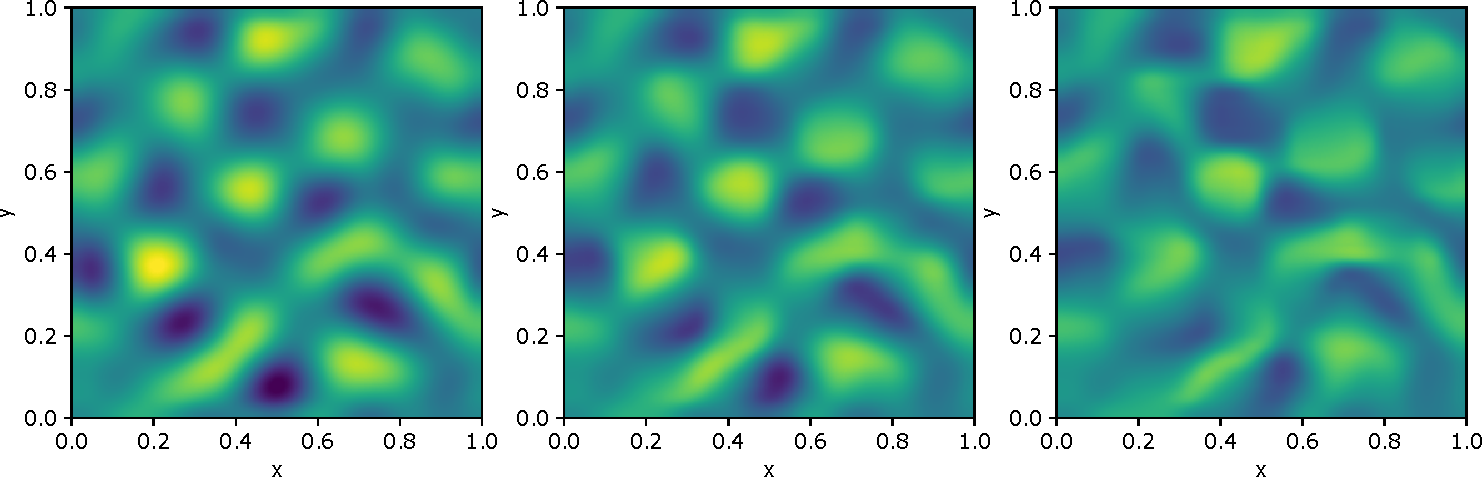
\includegraphics[scale=0.35]{ns_p_trim.pdf}
%          \caption{From left to right, states (in this case, density fields) $\state_{0}, \state_{1}, \state_{2}$ evolving through time.}
%          \label{fig:states}
%      \end{subfigure}
%      \begin{subfigure}{0.25\textwidth}
%          \centering
%         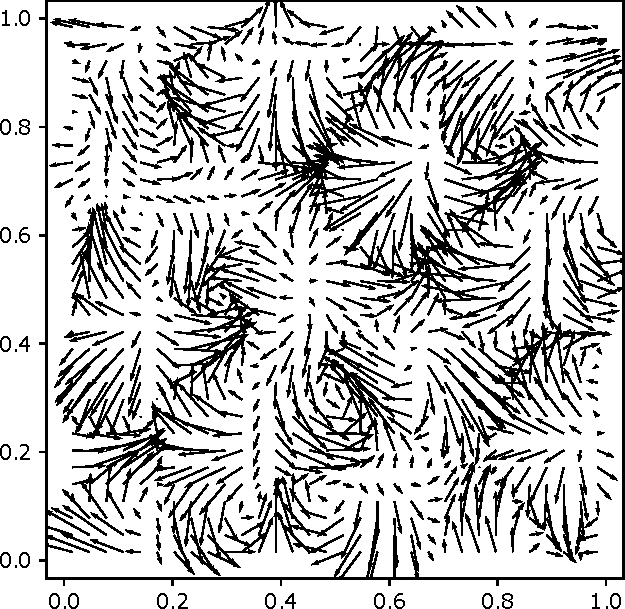
\includegraphics[scale=0.25]{ns_force_trim.pdf}
%          \caption{Unobserved parameter $\forcing$.}
%          \label{fig:forcing}
%      \end{subfigure}
%      \hfill
%     \centering
%     \caption{An example Navier-Stokes fluid flow system, used as a case study in this work. State and velocity vectors are projected into the original space representing the evolutions of a physical system.}
%     \label{fig:dynamicalsystem}
% \end{figure*}


% \section{Deterministic operator inversion}
\section{Approaches to model inversion}
We review some classical approaches to model inversion in \S \ref{sec:InversionMAP} - \S \ref{sec:InversionGP}, then present our new approach, \meth{}, in \S \ref{sec:EnsembleInversion}, and discuss hyperparameter selection in \S \ref{sec:HyperparamSelection}.

\subsection{Inversion by optimisation}\label{sec:InversionMAP}
One straightforward approach is to choose by optimisation a parameter estimate that minimises some discrepancy between the observation and the model prediction given the parameter, minimising some prediction loss.
If this loss arises from an observation likelihood we can frame this as likelihood maximisation.
Any
%(not necessarily unique)
\emph{maximum a posteriori} (MAP) estimate $\hat{\forcingst}$ satisfies
\begin{align*}
    \hat{\forcingst} \in \argmax\limits_{\forcingst \in \mathcal{U}}  \log
         p\big( \forcingst \gvn \mathcal{D}_t \big)
         + \log p(\forcingst).\numberthis \label{eq:pred_error_inv}
\end{align*}
\russ{This looks possibly wrong? Shouldn't the first term be a log likelihood? Also a negative sign?}



The optimisation problem described in (\ref{eq:pred_error_inv}) is often under-determined, in the sense the optimum may not be unique.
To make matters worse, gradient-based optimisation may converge to local, rather than global, maxima.
When the dimensionality $D_{\forcing}$ is large, traditional second order optimisation methods can become computationally intractable on account of the large linear systems that need to be solved.
Additionally, if the log-likelihood is non-convex in $\forcing$, most algorithms will only be able to find a local optimum of~\eqref{eq:pred_error_inv}.
Under certain conditions~\citep[Chapter 5]{WrightOptimization2021}, stationary points of~\eqref{eq:pred_error_inv} may be efficiently computed, even for high dimensional $D_{\forcing}$, by gradient descent or stochastic gradient descent~\citep{XuADCME2020,MacKinlayModel2021} of the negative log-likelihood function for a white-box forward model.
A downside of point estimates obtained by optimisation, is that they do not contain any uncertainty estimates for given solutions.
Efficient routines exist for computing uncertainty of point estimates via second order methods that exploit sparsity and variable ordering heuristics~\citep{DellaertFactor2017}, however an optimisation-based perspective is inherently limited to uncertainty quantification locally around the MAP estimate.

In the Bayesian setting, we can remedy issues associated with both non-convexity and lack of uncertainty information, using appropriate prior $p(\forcing)$ in~\eqref{eq:pred_error_inv} to regularise solutions towards \emph{a priori} plausible solutions, and assigning a posterior weight to various candidate solutions.
In the pure optimisation setting, we can also use regularisation to penalise the parameter-space towards plausible solutions, although inclusion of the regularisation term loses the intuitive interpretation that we gain from employing a prior.
%However, excessively large prior regularisation terms can lead to undesirable properties of the estimate, such as slower convergence to a true model parameter in the case of a well-specified model.

This approach can be generalised to a stochastic forward operator, by taking expectations
\begin{align*}
    \hat{\forcingst} :=\argmin_{\forcingst}
        \Ex_{\vrv{\nu}}[L\left(
            \statest_{t},
            \op{P}(\statest_{\tm}, \forcingst,\vrv{\nu})
        \right)].\numberthis \label{eq:pred_error_inv_stoch}
\end{align*}
Solution in that case may be estimated by stochastic gradient descent method. \russ{Monte Carlo gradient method == SGD and friends?}\danm{yes, but need to expand if we keep this bit in there.}

%\subsection{Naive Bayesian inversion}
%\label{sec:naive_bayes}

%\russ{I still don't understand the construction. Maybe my confusion is related to the lack of subscripts on $\mathsf{z}$ and $\mathsf{u}$, or maybe not. I general I cannot see how $\mathsf{z}$ is a Gaussian process is compatible with~\eqref{eq:proc_proj_sem_inv} holding. Maybe my confusion is related to what ``simple choice for probabilistic modelling" means. Maybe my confusion is related to whether $\mathsf{z}$ is Gaussian when indexed by time, space or both?}




\subsection{Bayesian inversion with linearised Gaussian processes}\label{sec:InversionGP}
\label{sec:error_prop}
Our goal is to approximate the posterior $p(\forcingst \gvn \mathcal{D}_t)$ using a Gaussian distribution $q(\forcingst \gvn \mathcal{D}_t)$ that admits an iterative update in terms of $q(\forcingst \gvn \mathcal{D}_{t-1})$.
To this end, define
\begin{align*}
    q(\forcingst \gvn \mathcal{D}_{t}) := \mathcal{N}(m_t, \Sigma_t) \approx p(\forcingst \mid \mathcal{D}_t), \numberthis \label{eq:approx_distribution}
\end{align*}
where $m_t \in \mathcal{U}$ and $\Sigma_t \in \mathbb{S}^{D_{\forcing}}_+$ are mean and covariance parameters.
We take $q(\forcingst\gvn\mathcal{D}_0)$ to be the (exact, unconditional) prior, $q(\forcingst\gvn\mathcal{D}_0)=p(\forcingst)$.

\paragraph{Linearisation of the forward operator} A classic choice is to define the mean and covariance parameters in terms of a linearised approximation to the forward operator of the system, \( \op{P}\).
This is the basic technique underlying the propagation of errors, the Extended Kalman Filter, and more generally, Gaussian Belief propagation  (e.g.~\citet{OrtizVisual2021}).
Specifically, for some expansion point \(\forcingst_0\), we make the linear approximation
\begin{align*}
    \state_t = \op{P}(\state_{\tm}, \forcing)
    &\approx\underbrace{
    \op{P}(\state_{\tm},\forcingst_0)
    + %\begin{bmatrix}
        % \mm{J}_{\state_{\tm}}\\
        \mm{J}_{\forcingst_0}
    % \end{bmatrix}
    % \begin{bmatrix}
        % \statest-\statest_{0}\\
        (\forcing-\forcingst_0)}_{:= \widehat{\op{P}}_{\forcingst_0}(\state_{\tm}, \forcing)},
    % \end{bmatrix},
    \numberthis \label{eq:linear_p}
\end{align*}
where
\begin{align*}
    % \mm{J}_{\state_{\tm}}&:=\left[\nabla_{\statest}\op{P}(\statest,\forcingst)\right]_{\statest=\state_{\tm}, \forcingst=\forcingst_0}\\
    \mm{J}_{\forcingst_0}&:=\left.\nabla_{\forcing}\op{P}(\state_{\tm},\forcingst)\right|_{\forcingst=\forcingst_0}.
\end{align*}
% are the Jacobian matrices associated with each argument.
% Collectively these motivate an approximate update rule.
%We use the linearised form \eqref{eq:linear_p} to approximate \eqref{eq:gaussian_approx_proc}, expanding about the prior mean
\paragraph{Approximation of the joint conditional}
We use the linearised form \eqref{eq:linear_p} to define the approximate conditional distribution of $\state_t$ and $\forcing$ given $\mathcal{D}_{t-1}$.
Setting
\(\forcingst_0=
m_{\tm}\), in this approximation, we find that the joint conditional distribution satisfies
\begin{align*}\left.
    \begin{bmatrix}
        \forcing \\ \state_{t}
    \end{bmatrix}\right| \mathcal{D}_{t-1}
    &\approxdisteq \left.
    \begin{bmatrix}
        \forcing \\
        \widehat{\op{P}}_{m_{t-1}}(\statest_{\tm},\forcing) +\vrv{\varepsilon}
    \end{bmatrix} \right| \mathcal{D}_{t-1} \numberthis\label{eq:ekf-linearisation}
\end{align*}
where \(\vrv{\varepsilon}\sim \dist{N}(0,\sigma^2\mm{I}\)) is a noise term that admits a degree of model misfit.

\paragraph{Updating the approximate posterior}
Under this approximation, the moments of the updated approximate density $q(\forcingst \mid \mathcal{D}_t)$ in the form \eqref{eq:cond-joint-normal} are given by
\begin{align*}
    {m}_{t}
        &= m_{t-1} + \emph{G} (\statest_t -  \widehat{\op{P}}_{m_{t-1}}(\statest_{\tm},m_{t-1})) \\
        \Sigma_t &= \Sigma_{t-1} - \emph{G}  J_{m_{\tm}} \Sigma_{t-1}
\end{align*}

\noindent where \( \emph{G} := \Sigma_{t-1}J_{m_{\tm}}^\top (J_{m_{\tm}} J_{m_{\tm}}^\top + \sigma^2 I)^{-1} \) is the gain matrix and the inverse is meant in a generalised sense.
The gain matrix $G$ may not need to be formed explicitly, although linear systems involving the gain matrix need to be solved.
\begin{align*}
    {m}_{\state_{t}}
        &=\op{P}(\statest_{\tm},\vv{m}_{\forcingst})\numberthis\label{eq:linear-p-state-mean}\\
    \mm{K}_{\state_{t}\state_{t}}
         &=J_{{m}_{\forcingst}}\mm{K}_{\forcing\forcing}J_{{m}_{\forcingst}}^{\top} +\sigma^2\mm{I}\numberthis \label{eq:linear-p-state-cov}\\
    \mm{K}_{\state_{t}\forcing}
    % \mm{K}_{\statest\forcingst}{}
        &=\mm{K}_{\forcing\forcing}J_{{m}_{\forcingst}}^{\top}\numberthis \label{eq:linear-p-cross-cov}
\end{align*}
since \(\widehat{\op{P}}\) is linear.
% We can envisage this as a variational approximation, where the posterior mean and variance are chosen to minimise a KL-divergence between a true posterior and the local posterior approximation.\nb{write out KL-divergence version?}
This provides a recipe for iteratively updating beliefs about \(\forcing\) given new observation pairs \(\state_{\tm}{=}\statest_{\tm},\state_{t}{=}\statest_{t} \) by iteratively applying \eqref{eq:cond-joint-normal} to the moments arising from linearised approximation~\eqref{eq:ekf-linearisation}.
%Given some prior distribution for \(\forcing\) we can estimate \(\state_{t}\gvn (\state_{\tm}{=}\statest_{\tm},\forcing{=}\forcingst)\) using the linearised \eqref{eq:ekf-linearisation}, so that the observation likelihoods may be put into conditionally-jointly-normal form \eqref{eq:cond-joint-normal}, with moments given in terms of the Jacobian of the operator as per \eqref{eq:linear-p-state-mean}--\eqref{eq:linear-p-cross-cov}.
%Next, we can update our estimates for the posterior moments of \(\forcing\) by applying \eqref{eq:gaussian-cond-mean} and \eqref{eq:gaussian-cond-cov}.

This gives an update for the parameters $m_t$ and $\Sigma_t$ of $q(\forcingst \gvn \mathcal{D}_t)$ in terms of the parameters $m_{t-1}$ and $\Sigma_{t-1}$ of the previous density $q(\forcingst \gvn \mathcal{D}_{t-1})$ and observation $\statest_t$.

This approach can produce inferior results for problems where the action of the forward operator is not well-summarised by a linear transformation about the mean.
In practice for nonlinear models this means that the value of \(\sigma^2\) plays a role in reducing the influence of new observations and increasing the stability of updates.
Linearisation also performs unfavourably in high-dimensional problems.
The storage requirements of the  posterior statistics are large, comprising a mean function and also a covariance matrix between all sites, necessitating updating a \(D_{\forcing}\times D_{\forcing}\) covariance matrix.
Further, computing this update can be  expensive, as the updates in \eqref{eq:gaussian-cond-var} and \eqref{eq:gaussian-cond-mean} require solving a linear system, which incurs a \(\mathcal{O}(D_{\vrv{\state}}^3)\) computational time cost.
Moreover, the capacity of this model to handle non-deterministic predictions is limited, since only linearly additive noise may be easily applied to the prediction model.
In the next section we attempt to address these problems simultaneously using an ensemble sampling method.

\subsection{Our solution: ensemble inversion via \meth{}}\label{sec:EnsembleInversion}

% \begin{figure*}[h!t]
%      % \centering
%     \begin{subfigure}{0.3\textwidth}
%          % \centering
%         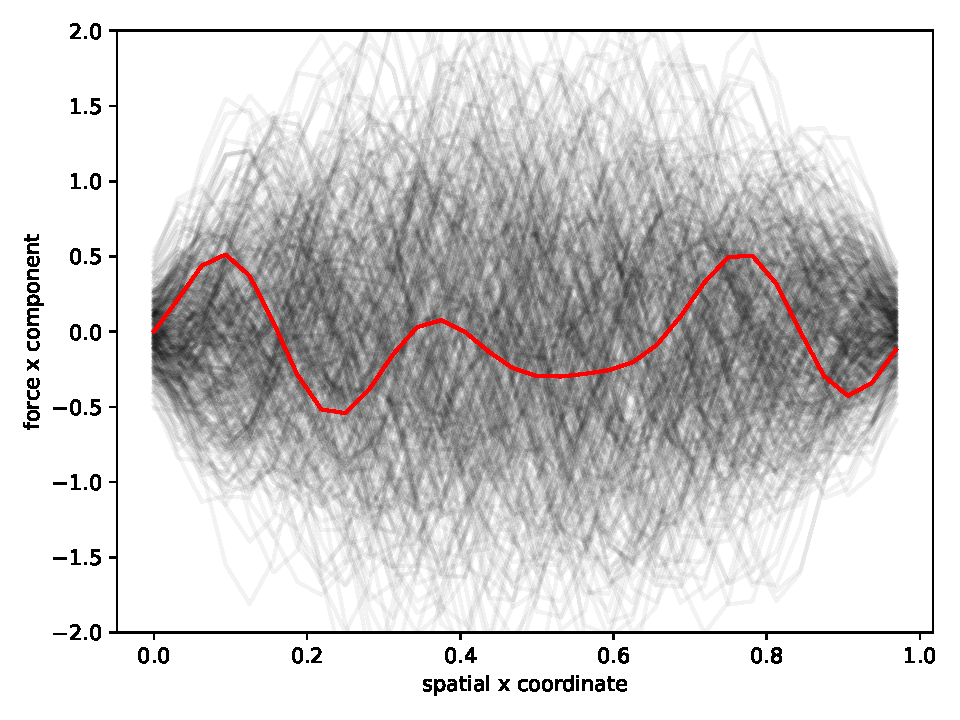
\includegraphics[scale=0.35]{meth_ex_guess_0.pdf}
%          \caption{Prior samples of \(\forcing\)}
%          \label{fig:meth_ex_0}
%     \end{subfigure}
%     \begin{subfigure}{0.3\textwidth}
%          % \centering
%         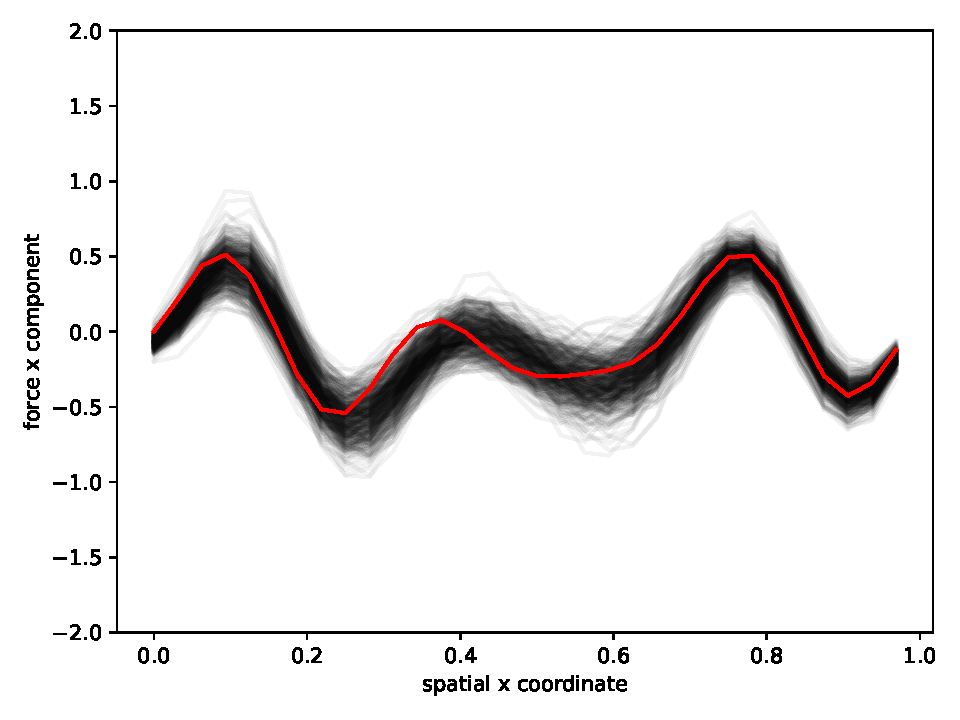
\includegraphics[scale=0.35]{meth_ex_guess_1.pdf}
%          \caption{\meth{} samples \(\forcing\gvn \state_0,\state_1\).}
%          \label{fig:meth_ex_1}
%     \end{subfigure}
%     \begin{subfigure}{0.3\textwidth}
%          % \centering
%         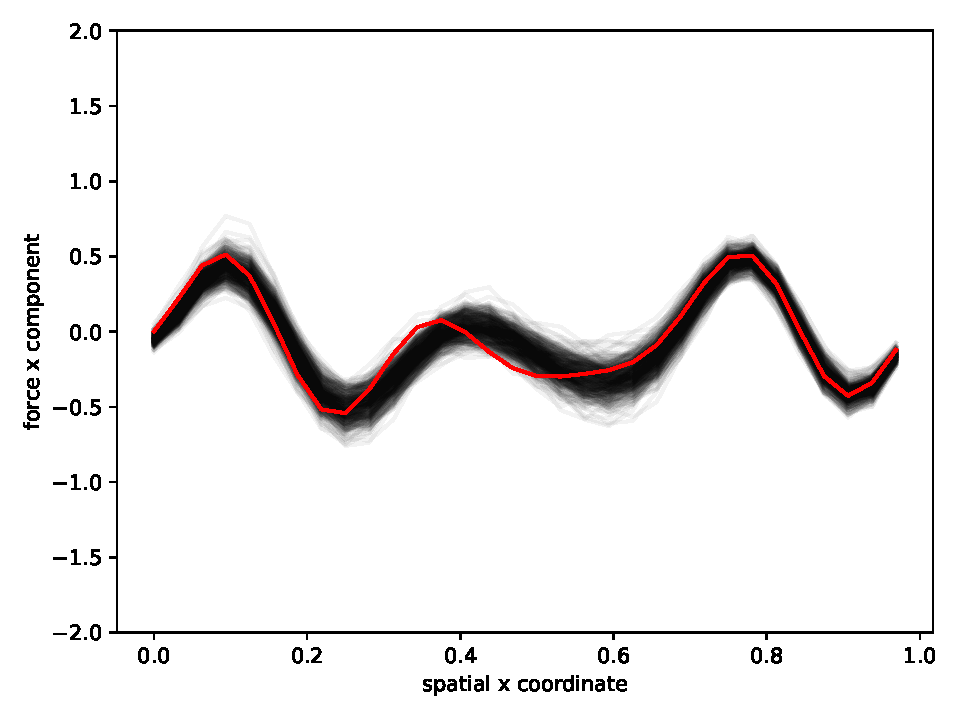
\includegraphics[scale=0.35]{meth_ex_guess_4.pdf}
%          \caption{\meth{} samples \(\forcing\gvn \state_0,\cdots\state_5\).}
%          \label{fig:meth_ex_4}
%      \end{subfigure}
%      \hfill
%     \centering
%     \caption{A slice along the \(x\) spatial  axis of  \(N=400\) sampled solutions computed via \meth{}. The solid red line shows ground truth, and each transparent grey line is one sample from the solution space.}
%     \label{fig:inverse-slices}
% \end{figure*}


The aforementioned limitations of the linearised propagation of errors can be eased by moving to Monte Carlo inference, wherein distributions are no longer summarised by their moments but  by samples drawn from those distributions.
Specifically, our method, \meth, is related to the family of Ensemble Kalman methods of Data Assimilation~\cite{EvensenData2009} and their generalisation to solve inverse problems~\cite{IglesiasEnsemble2013}.
Unlike the linearised version, ensemble methods are applicable to black-box models and stochastic models.  They summarise all random variates through an ensemble of (possibly approximate) samples from the distribution of that random variate.
The price for this is a need to execute the forward model more times (once for each ensemble member), with ensemble sizes typically in the order of hundreds.

In typical Gaussian inference we perform  an update by applying Bayes' rule to the distributions of the random variates involved, e.g. integrating the densities in~\eqref{eq:bayes_rule}, or in the case of conjugate models by updating moments of the belief distribution as per~\eqref{eq:cond-joint-normal}.
An ensemble-wise Gaussian eschews either of these in favour of perturbing the empirical distribution induced by samples in our ensemble.
That is, the \emph{empirical} ensemble moments satisfy the data-conditional update formula~\eqref{eq:cond-joint-normal}.
We use the Matheron update~\citep{WilsonPathwise2021} to perform the perturbation without evaluating the intermediate densities or forming covariance matrices.

Each sample from the prior belief distribution is perturbed so that the perturbed ensemble represents approximately independent samples from the posterior distribution conditional on the observations.
Such methods are frequently more computationally efficient and flexible than the error-propagation method of section \ref{sec:error_prop}, which acts directly upon the sufficient statistics of the Gaussian distribution rather than samples.
Further, ensemble methods are widely understood to attain superior performance in non-linear systems~\citep{FearnheadParticle2018}.
\meth{} is precisely the application of this method to the inference of hidden parameters rather than model states as in classical filtering.

%\russ{I think I am confused about what should be bold or not bold like $\forcing$ or $\forcingst$.}
%What is a random variable and what is a sample? https://stats.stackexchange.com/questions/368492/about-sampling-and-random-variables
\paragraph{Ensemble of parameters and states}
In  \meth{}, we begin by sampling from the prior distribution for \(\forcing \sim p(\forcingst)\) independently $N$ times.
We write the samples as
\begin{align*}
    \mm{U}_{0}= \begin{bmatrix}
        \forcingst_{0}^{(1)}, & \cdots, & \forcingst_{0}^{(N)}
    \end{bmatrix} \in \mathbb{R}^{D_{\forcing}\times N}.
\end{align*}


Our goal is to successively update this ensemble, constructing new ensembles  such that their columns contain samples from an approximate posterior $\forcing \sim \rho(\forcingst \gvn \mathcal{D}_t)\approx p(\forcingst \gvn \mathcal{D}_t)$. We similarly write such samples as
\begin{align*}
    \mm{U}_{t}=\begin{bmatrix}\forcingst_{t}^{(1)}, & \cdots, & \forcingst_{t}^{(N)} \end{bmatrix} \in \mathbb{R}^{D_{\forcing}\times N}.
\end{align*}
We now define the approximate posterior $\rho(\forcingst \gvn \mathcal{D}_t)$.  Mirroring the moment-centric approximation~\eqref{eq:approx_distribution}, we introduce an ensemble-centric approximation  with parameters replaced by empirical estimates of parameters,
$$\rho(\forcingst \gvn \mathcal{D}_t) := \dist{N}(\overline{\mm{U}}_t,\breve{\mm{U}}_t\breve{\mm{U}}^{\top}_t+ \tau^2\mm{I}) \approx p(\forcingst \gvn \mathcal{D}_t), $$
where empirical means and empirical variances are
\begin{align*}    %\widehat{\Ex}
    \overline{\mm{U}}_t:=\frac{1}{N}\sum_{i=1}^N \forcingst^{(i)}_t\quad  \text{and} \quad
    \widehat{\var}(\mm{U}_t)&:=\breve{\mm{U}}_t\breve{\mm{U}}^{\top}_t,
\end{align*} where
\begin{align*}
\breve{\mm{U}}_t&:={\textstyle\frac{1}{\sqrt{N-1}}}\begin{bmatrix}
    (\forcingst^{(1)}_t-\overline{\mm{U}}_t) & \cdots & (\forcingst^{(N)}_t-\overline{\mm{U}}_t)
\end{bmatrix}.
\end{align*}
The breve-marked matrices \(\breve{\mm{U}}_t\) we call \emph{deviation matrices}.
%$$\forcing_t\sim \dist{N}(\overline{\mm{U}},\breve{\mm{U}}\breve{\mm{U}}^{\top}+ \tau^2\mm{I}). $$
The additional \(\tau^2\) term is introduced to explicitly admit a degree of model misfit;
since the ensemble spans a \(N\)-dimensional subspace of the overall solution space by construction, the likelihood will be 0 for observations which deviate from that subspace even minutely.
%\textcolor{blue}{We return to this theme momentarily.}

Given an ensemble \(\mm{U}_{\tm}\) and observation $\statest_{t-1}$, we construct a predictive ensemble for the state at the next timestep,
\begin{align*}
    \mm{Z}_{t}&= \begin{bmatrix}
        \op{P}(\statest_{\tm},\forcingst_{\tm}^{(1)}) & \cdots & \op{P}(\statest_{\tm},\forcingst_{\tm}^{(N)})
    \end{bmatrix}\\
    &=:\begin{bmatrix}
        \statest^{(1)}_t & \cdots & \statest^{(N)}_t
    \end{bmatrix}. \numberthis \label{eq:predictive_ensemble}
\end{align*}
We define the empirical ensemble means,
\begin{align*}
    %\widehat{\Ex}
    \overline{\mm{Z}}:=\frac{1}{N}\sum_{i=1}^N \statest^{(i)}\\
    \overline{\mm{U}}:=\frac{1}{N}\sum_{i=1}^N \forcingst^{(i)}
\end{align*}
and empirical ensemble variances in terms of deviation matrices
\begin{align*}
    \widehat{\var}(\mm{Z})&=\breve{\mm{Z}}\breve{\mm{Z}}^{\top}\\
    \widehat{\var}(\mm{U})&=\breve{\mm{U}}\breve{\mm{U}}^{\top}
\end{align*} where
\begin{align*}
\breve{\mm{Z}}&={\textstyle\frac{1}{\sqrt{N-1}}}\begin{bmatrix}
    (\statest^{(1)}-\overline{\mm{Z}}) & \cdots & (\statest^{(N)}-\overline{\mm{Z}})
\end{bmatrix}\\
\breve{\mm{U}}&={\textstyle\frac{1}{\sqrt{N-1}}}\begin{bmatrix}
    (\forcingst^{(1)}-\overline{\mm{Z}}) & \cdots & (\forcingst^{(N)}-\overline{\mm{U}})
\end{bmatrix}.
\end{align*}
\paragraph{Ensemble approximation of the joint conditional}
Together, the joint ensembles $\mm{U}_{t-1}$ and $\mm{Z}_{t}$ represent $N$ samples from an approximate joint conditional distribution.
We make the approximation that the conditional $\forcing, \state_t \gvn \mathcal{D}_{t-1}$ is jointly Gaussian, so that
\begin{align*}& \left.
\left[\begin{array}{c}
    \forcing \\
    \state_{t}
\end{array}\right] \right| \mathcal{D}_{t-1} \numberthis\label{eq:discrete_joint_enkf_sim} \\
    &\sim \dist{N}\left(
    \left[\begin{array}{c}
        \overline{\mm{U}}_{\tm} \\
        \overline{\mm{Z}}_{t}
    \end{array}\right],
    \left[\begin{array}{cc}
        \breve{\mm{U}}_{\tm}\breve{\mm{U}}_{\tm}^{\top} + \tau^2\mm{I}
        &  \breve{\mm{Z}}_{t}\breve{\mm{U}}_{\tm}^{\top} \\\ % 3 backslashes or it breaks for some reason
        \breve{\mm{U}}_{\tm}\breve{\mm{Z}}^{\top}_{t}
        & \breve{\mm{Z}}_{t}\breve{\mm{Z}}_{t}^{\top} +\sigma^2\mm{I}
    \end{array}\right]\right).%\\
\end{align*}
The noise terms, \(\sigma^2\) and \(\tau^2\), act to diffuse observation and posterior likelihoods respectively, to account for model misspecification, as in the \(\sigma^2\) in the linearised Gaussian approximation.
Given this approximated joint distribution, we must update the ensemble to sample from the conditional ${\rho(\forcingst \gvn \mathcal{D}_t)}$.
To that end, we employ a pathwise variant of the update performed in \S~\ref{sec:error_prop}.



\paragraph{Updating the ensemble} We now employ the Matheron update.
Suppose we make a new observation $\state_t = \statest_t$ on which we would like to condition.
Combining~\eqref{eq:matheron_rule_1} with~\eqref{eq:discrete_joint_enkf_sim}, random variables following the conditional distribution with conditional density $\rho(\forcingst \gvn \mathcal{D}_t)$ satisfy the following relation to random variables following the conditional joint density $\rho(\forcingst, \statest_t \gvn \mathcal{D}_{t-1})$,
\begin{align*}
    \forcing \mid \mathcal{D}_t \stackrel{d}{=}
    \forcing
    + \breve{\mm{Z}}_{t}\breve{\mm{U}}_{\tm}^{\top}
    \left(\breve{\mm{Z}}_{t}\breve{\mm{Z}}_{t}^{\top}+\sigma^2\mm{I}\right)^{-1}
    \left(
        \state_{t}-\statest_{t}
    \right)\numberthis\label{eq:pathwise-update}.
\end{align*}
Since we already possess samples from the conditional joint density $\rho(\forcingst, \statest_t \gvn \mathcal{D}_{t-1})$, in $\mm{U}_{t-1}$ and $\mm{Z}_t$, we perform an update by inserting them in place of $\forcing$ and $\state_t$ in~\eqref{eq:pathwise-update}.
This results in a new ensemble $\mm{U}_t$, from which a predictive ensemble $\mm{Z}_{t+1}$ is constructed by applying~\eqref{eq:predictive_ensemble}, and so the procedure continues.
A summary of the \meth{} algorithm presented as pseudocode, is given in Appendix~\ref{app:algorithm}.

% In the case that \(\op{P}\) is linear, this is exact.
% and such an update maps individual prior samples of \(\forcing\) to individual posterior samples \(\forcing\gvn (\state_{\tm}=\statest_{\tm},\state_{t}=\statest_{t})\).
The update~\eqref{eq:pathwise-update} may be calculated efficiently and in parallel using the Woodbury identity and Cholesky decomposition, and wihtout constructing the \(D_{\forcing}\times D_{\forcing}\) covariance matrix of the conditional distribution of \(\forcing\) in order to find the update (see \S~\ref{sec:computational_cost}).
All operations may be conducted in terms of the \(D_{\forcing}\times N\) deviance matrices, where typically \(D_{\forcing}\gg N\).
By recursive application of \eqref{eq:pathwise-update}, we iteratively assimilate observations to sample from the target posterior.

\subsection{Hyperparameter selection}\label{sec:HyperparamSelection}
Hyperparameters \(\sigma^2\) and \(\tau^2\) can be interpreted as residual prediction noise, arising from stochastic perturbation or model misfit.
Alternatively, we can interpret them as smoothing applied to ensure numerical stability of the updates.
As residual prediction noise, they may be notionally estimated by, for example, the method of maximum likelihood~\citep{MitchellAdaptive2000}.
In practice, we choose the pragmatic interpretation of these parameters as choices we can use to ensure numerical stability of the algorithms.
Increasing \(\sigma^2\) reduces the size of the posterior update from each new observation, reflecting how uncertain we are about our method.
Increasing \(\tau^2\) increases the posterior variance of the estimate of \(\vrv{u}\) since the likelihood may be zero evaluated at points which do not fall exactly on the subspace spanned by the members of the ensemble \(\mm{U}\).
We fix \(\tau^2=10^{-4}\) throughout.
For \meth{} we fix \(\sigma^2=10^{-4}\).
For the linearised Gaussian method, we use a brute-force search to find the smallest value such that updates rarely diverge after the first update step, settling upon \(\sigma^2=0.1\).

\subsection{Computational cost}
\label{sec:computational_cost}
\paragraph{Linearised Gaussian process} In the method of linearisation (\S~\ref{sec:error_prop}), the dominant time cost in inference is the solution of the linear system defined by the covariance matrix in order to calculate the effect of the gain.
Even exploiting positive definiteness, this operation in general scales as \(\mathcal{O}\left(D_{z}^3\right)\).
The cost of calculating the model Jacobian can depend upon the model, but for many models is linear in the dimension of the Jacobian, and so the simulation cost per time step scales as \(\mathcal{O}\left(D_{\state}\right)\).

\paragraph{\textbf{METHO}} In the ensemble method, the cost of running simulations is simply \(\mathcal{O}\left(N\right)\) the ensemble size.
During the inference stage the dominant cost is once again solving the linear system to calculate the gain matrix.
We may exploit the ensemble structure to solve the linear system in the update efficiently.
Suppose \(\mm{K}_{zz}=\breve{\mm{Z}} \breve{\mm{Z}}^{\top}+\sigma^2\mm{I}\).
Applying the Woodbury identity,
\begin{align*}
\mm{K}_{zz}^{-1}=\sigma^{-2}\mm{I}-\sigma^{-4} \breve{\mm{Z}}\left(\mm{I}+\sigma^{-2}\breve{\mm{Z}}^{\top}  \breve{\mm{Z}}\right)^{-1} \breve{\mm{Z}}^{\top}.
\end{align*}
We compute the (lower triangular, unique) Cholesky decomposition \(\mm{L} \mm{L}^{\top}=\left(\mm{I}+\sigma^{-2}\breve{\mm{Z}}^{\top} \breve{\mm{Z}}\right)^{-1}\) at a cost of $\mathcal{O}(N^3)$, and define \(\mm{R}=\sigma^{-2}\breve{\mm{Z}} \mm{L}\).
We use this to discover
\[
\mm{K}_{zz}^{-1}=\sigma^{-2}\mm{I}-\mm{R} \mm{R}^{\top},
\]
and then compute the solution of a linear system involving $\mm{K}_{zz}$ through multiplication.
The solution of the linear system is thus \(\mathcal{O}\left(N^2 D_{\state}+N^3\right)\).
This cost is favourable in comparison with $\mathcal{O}(D_{\state})$ when $N < D_{\state}$.

\section{Experiments}


\subsection{Deterministic Navier-Stokes}
% \begin{figure}[h!t]
%     \centering
%     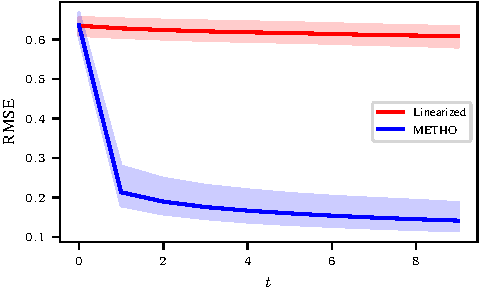
\includegraphics[scale=1]{linear_vs_metho_large.pdf}
%     \centering
%     \caption{Recovery of latent forcing in a Navier-stoke inversion problem. The plotted RMSE is unweighted \(\ell_2\) distance between MAP estimate \(\argmax \rho(\forcingst \gvn \mathcal{D}_t)\) and ground truth \(\forcingst\). Colored region denotes 90\% band over 80 realisations.}
%     \label{fig:linear_vs_metho}
% \end{figure}

We use a Navier-Stokes flow model on a 2-dimensional square domain with Neumann boundary conditions and inhomogenous forcing as depicted in Figure~\ref{fig:dynamicalsystem}.
The solver in this case has an heterogeneous acceleration term representing an external driving term \(\vrv{\forcing}\).
Both initial conditions and latent forcings are drawn from stationary Gaussian random fields with exponentially decaying spectrum.
Initial velocities are multiplied by an envelope term to ensure they satisfy Neumann boundary conditions.
For details see Appendix~\ref{app:pdes}.

In the deterministic setting the model is completely determined by initial conditions and latent parameters, and we may apply the method of linearisation to recover estimates of the unknown \(\vrv{\forcing}\).

We apply \meth{} with an ensemble size of 400, \(\sigma^2=10^{-4}\) and the linearised method with \(\sigma^2=0.1\), and compare each method in terms of the \(\ell_2\) error between the MAP estimate and ground truth, on a spatial grid of size \(128\times 128\).
Results are plotted in Figure~\ref{fig:linear_vs_metho}.
Although both are able to iteratively improve the error in this metric, the linearised method is drastically less data-efficient in that the solution improves less with each time step, as we would expect for a large \(\sigma^2\).
On the other hand, setting \(\sigma^2\) to a smaller number results in unstable inference, with solutions not improving or even diverging.

Timings reflect inference on NVIDIA P100 GPUs, implemented in pytorch.
The 90\% range of simulation time (i.e. running the prediction model) for the linearised method was $18$-$24$ seconds and for \meth{} was $2.6$--$3$ seconds.
We note, however, that the linearised method is possibly unfairly penalised by the inefficient implementation of multivariate Jacobians in the version of pytorch used.
The 90\% range for the inference time for the linearised method in was $0.13$-$0.26$ seconds and for the \meth{} was $0.027$--$0.064$ seconds.

\subsection{Stochastic Navier-Stokes}

In the stochastic case the Navier-Stoke solver is perturbed by adding a spatially homogeneous, centred, white Gaussian noise \(\vrv{\nu}_t\) term to the each element of the velocity vector before applying the forward prediction operator of the Navier-Stoke solver.
In this stochastic setting we cannot apply the linearised method.
Moreover, in this problem the solution grid is of dimension \(512 \times 512\), which causes the covariance matrices to be too large for inference on common hardware.

In this challenging setting we test the influence of the ensemble size upon the quality of \meth{} inference.
For each ensemble size we conduct 80 replicates over 5 observation updates.
Results are plotted in Figure~\ref{fig:n_ens}.

Because the likelihood (and therefore the posterior) is not ever explicitly formed in this black-box forward model and is in any case intractable, it is difficult to evaluate the exact posterior density assigned to the ground truth parameter $\forcingst^\ast$.
That is, we cannot evaluate $p(\forcingst^\ast \gvn \mathcal{D}_T)$.
However, all else being equal, assigning a high value to the approximate posterior density $\rho(\forcingst^\ast \gvn \mathcal{D}_T)$ evaluated at $\forcingst^\ast$ is indicative of a higher quality model.
In Figure~\ref{fig:n_ens} we plot $\rho(\forcingst^\ast \gvn \mathcal{D}_t)$ as a function of ensemble size $N$.
We see a gradual improvement then plateau in all metrics as the size of the ensemble grows, although selecting the precise trade-off is problem-dependent.


% \begin{figure}[h!t]
%     \centering
%      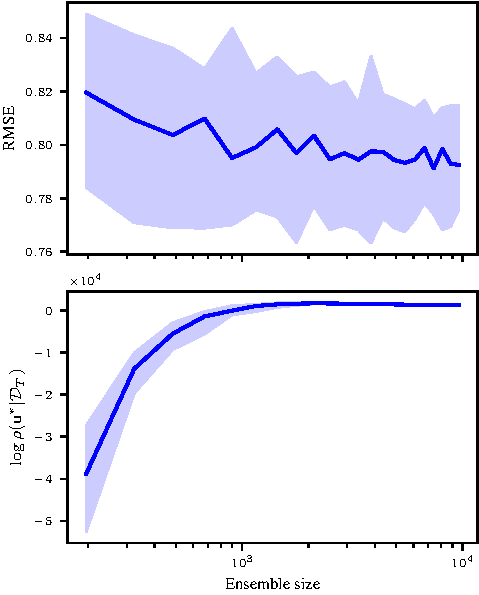
\includegraphics[scale=1]{meth_ex_ens_5.pdf}
%     \centering
%     \caption{Effect of ensemble size on model RMSE and estimated likelihood. 80 replicates of 5 observations, i.e. \(T=4\). Shaded region shows empirical 90\% range, dark line shows median.}
%     \label{fig:n_ens}
% \end{figure}


\section{Conclusion}

\meth{} is an easy-to-implement and flexible method enabling inverse inference with challenging observation models.
Sample-based conditional updates are an under-utilised technique in machine learning.
Although their use in time-series filtering is well-known, their use in inverse problems is less appreciated.
We hypothesise there are more useful techniques to be uncovered here.
Bringing the Machine Learning research on pathwise updates into engagement with the Ensemble method literature suggests improvements to each.
For example, outside the ensemble context, \citet{WilsonPathwise2021} observe that Matheron updates are very general and may be extended from finite vectors to continuous functions spaces, even to processes on smooth manifolds other than \(\mathbb{R}^{D}\) by Karhunen-Lo\`eve expansions.
As with ensemble  filtering problems, ensemble inversion methods could possibly be accelerated by improved sampling schemes, for example with sigma-point or QMC sampling schemes.


\clearpage
\bibliographystyle{icml2023}
\bibliography{refs.bib}


\appendix
\onecolumn
\section{Matheron updates}\label{app:matheron}
The pathwise Gaussian process update (\emph{Matheron update}), credited to unpublished works of Matheron~\citep{WilsonPathwise2021,DoucetNote2010} is a method of simulating from a conditional of some jointly Gaussian variate.
The Matheron update \(\pi\) for a partitioned Gaussian random vector
\(\begin{bmatrix} \vrv{y} &\vrv{w}
\end{bmatrix}^{\top}\) is a mapping
\begin{align*}
\pi: \left(\vv{y},\vv{w};\Law\left(\begin{bmatrix}\vrv{y}\\\vrv{w}\end{bmatrix}\right) \right)\mapsto \vv{y}'
\end{align*}
such that
\begin{align*}
\begin{bmatrix}\vrv{y}\\\vrv{w}\end{bmatrix}&\sim \Law\left(\begin{bmatrix}\vrv{y}\\\vrv{w}\end{bmatrix}\right) \\
&\Rightarrow\\
\pi\left(\vrv{y},\vv{w};\Law\left(\begin{bmatrix}\vrv{y}\\\vrv{w}\end{bmatrix}\right) \right) &\stackrel{d}{=}  \vrv{y}\gvn (\vrv{w}{=}\vv{w}) .\numberthis\label{eq:matheron-prop}
\end{align*}
Where the joint distribution of the random variates is clear from context we suppress the third argument of the function \(\pi\).
\russ{In the last equation (not first), there are three typesettings $\vrv{w}, w$ and $\vv{w}$, but I think we only need 2, right? $\vrv{w}$ and $w$?}\danm{yes, we have alternated between \(\vv{w}\) and \(w\) throughout this whole document; that needs fixing everywhere. I think dan P has been standardising on \(\vv{w}\)} \russ{Also shouldn't $\pi$ have 3 arguments, because it accepts both $\vrv{w}$ and $w$ as an input?} \danm{oh yeah it should, I mean, depending on how we wish to phrase; the distributions could be absorbed into \(\pi\). it should act on two distributions ( a joint distribution, really) and an observation. How does current phrasing look? Other thought, though: we are already doing a non-standard presentation of the update rule; should we save this weird phrasing for some future paper where we exploit the generality?}

Such a rule is known for Gaussian RVs \begin{align*}
    \begin{bmatrix}\vrv{y}\\ \vrv{w}
\end{bmatrix}\sim\mathcal{N}\left(\begin{bmatrix}
    m_{\vrv{y}}\\ m_{\vrv{w}}
\end{bmatrix},\begin{bmatrix}
    \mm{K}_{\vrv{y}\vrv{y}} & \mm{K}_{\vrv{y}\vrv{w}} \\
    \mm{K}_{\vrv{w}\vrv{y}} & \mm{K}_{\vrv{w}\vrv{w}}
\end{bmatrix}\right).
\end{align*}
Since these variates are jointly Gaussian, the conditional is also Gaussian and a necessary and sufficient condition for the update rule may be written in terms of the first two moments of the conditional as
\begin{align*}
    %\Ex [\pi(\vrv{y},\vv{w}) )]
    %&=
    \Ex[\vrv{y}\gvn \vrv{w}{=}w]
    &=m_{\vrv{y}}
        +\mm{K}_{\vrv{w}\vrv{y}} \mm{K}_{\vrv{w}\vrv{w}}^{-1}(w-m_{\vrv{w}})  &\text{ first moment}\numberthis \label{eq:app-gaussian-cond-mean}\\
    %\var [\pi(\vrv{y},\vv{w}) )]
    %&=
    \var[\vrv{y}\gvn \vrv{w}{=}w]
    &=\mm{K}_{\vrv{y}\vrv{y}}
        -\mm{K}_{\vrv{w}\vrv{y}} \mm{K}_{\vrv{w}\vrv{w}}^{-1}\mm{K}_{\vrv{y}\vrv{w}}. &\text{ second moment}\numberthis \label{eq:app-gaussian-cond-var}
\end{align*}
The Gaussian Matheron update which satisfies \eqref{eq:matheron-prop} is
\begin{align*}
\pi: \left(\vv{y},\vv{w};\mathcal{N}\left(\begin{bmatrix}
    m_{\vrv{y}}\\ m_{\vrv{w}}
\end{bmatrix},\begin{bmatrix}
    \mm{K}_{\vrv{y}\vrv{y}} & \mm{K}_{\vrv{y}\vrv{w}} \\
    \mm{K}_{\vrv{w}\vrv{y}} & \mm{K}_{\vrv{w}\vrv{w}}
\end{bmatrix}\right)\right) \mapsto
\vv{y}+\mm{K}_{\vrv{w}\vrv{y}} \mm{K}_{\vrv{w}\vrv{w}}^{-1}\left[\vv{w}-\vrv{w}\right].\numberthis\label{eq:pathwise-update-disc-app}
\end{align*}
\russ{I think this should be 3 argument version, as above? In particular, it should not involve ${m}_{\vrv{w}}$. }\danm{certainly should not; updated. Although this notation still feels not quite right. are we `covertly' randomising over \(\vrv{w}\)? or is it plain enough? }
Note that this update does not require us to calculate \(\mm{K}_{\vrv{y}\vrv{y}}\)
and further, may be conducted without needing to evaluate the density of the observation.

The Matheron update is used, for example, in~\citep{WilsonEfficiently2020} for the case that we have a Gaussian observation operator \(\op{T}: \vrv{y} \mapsto \mm{T}\vrv{y} + \vv{b} + \vrv{z}\) with \(\mm{T}\) linear, \(\vv{b}\) deterministic, and \(\vrv{z}\sim\mathcal{N}(0,\mm{K}_{\vrv{z}})\), resulting in joint distribution
\begin{align*}
\begin{bmatrix}
\vrv{y}\\ \vrv{w}
\end{bmatrix} =
\begin{bmatrix}
\vrv{y}\\ \mm{T}\vrv{y} + \vv{b} + \vrv{z}
\end{bmatrix}\sim\mathcal{N}\left(
\begin{bmatrix}
    m_{\vrv{y}}\\ \mm{T}m_{\vrv{y}} + \vv{b}
\end{bmatrix},\begin{bmatrix}
    \mm{K}_{\vrv{y}\vrv{y}} & \mm{K}_{\vrv{y}\vrv{y}}\mm{T}^{\top} \\
    \mm{T}\mm{K}_{\vrv{y}\vrv{y}} & \mm{T}\mm{K}_{\vrv{y}\vrv{y}}\mm{T}^{\top}+\mm{K}_{\vrv{z}}
\end{bmatrix}\right).
\end{align*}
In such cases, \eqref{eq:pathwise-update-disc-app} becomes
\begin{align*}
\pi(\vv{y},\vv{w})
&=\vrv{y}+\mm{T}\mm{K}_{\vrv{y}\vrv{y}} \left(\mm{T}\mm{K}_{\vrv{y}\vrv{y}}\mm{T}^{\top}+\mm{K}_{\vrv{z}}\right)^{-1}\left[\vv{w}-\mm{T}m_{\vrv{y}}-\vv{b}\right].\numberthis\label{eq:matheron-linear-obs}
\end{align*}

% \russ{I don't understand the motivation for this. If I understand correctly, Matheron update is a solution to an optimisation problem. This optimisation problem is not ``linear least squares'' in the traditional sense, since it involves just matching the coordinates of the vector, not solving a linear system. In this sense, it is trivial because any vector $b$ admits a representation $b = \argmin_a \Vert a - b \Vert^2$, or more generally $b = \argmin_a D(a,b)$ where $D$ is nonnegative and zero iff $a=b$.}
% \danm{You're right this does not add anything non-trivial. I was hoping that this would be neater than the previous version of this appendix, but this method is not The Way,}

In this work, we suppose that the joint distribution of \(\begin{bmatrix} \vrv{y} &\vrv{w}\end{bmatrix}^{\top}\) arises from a nonlinear, stochastic operator \(\op{T}\) such that \(\op{T}\vrv{y}=\vrv{w}\).
We want to construct an approximate analogue to the Matheron update which  updates the ensemble samples so that their empirical \emph{ensemble} statistics approximately satisfy \eqref{eq:app-gaussian-cond-mean} and \eqref{eq:app-gaussian-cond-var}.
We hope this can work if we generalise the basic Matheron rule in two senses:
\begin{enumerate}
    \item An ensemble version, which rather than acting upon the first 2 moments of our prior belief distribution, should act upon an \emph{ensemble of samples} drawn from the prior belief distribution, which is
    \item applicable for nonlinear and stochastic \(\op{T}\)
\end{enumerate}
This is essentially the setting of the stochastic Ensemble Kalman filter~\citep{EvensenData2009} (EnKF).

Rewriting \eqref{eq:app-gaussian-cond-mean} and \eqref{eq:app-gaussian-cond-var} in terms of moments of this general \(\op{T}\vrv{y}=\vrv{w}\),
% If
% \(\Law(\vrv{y}')= \Law(\vrv{y}\gvn \vrv{w}{=}w)\) and moreover \(\op{T}\vrv{y}=\vrv{w}\) and they  were Gaussian rvs,
% then we could completely characterise the relationship via
\begin{align*}
    \Ex [\vrv{y}']
    &= \Ex[\vrv{y}\gvn \op{T}\vrv{y}{=}w]\\
    &=\Ex[\vrv{y}]
        +\var[\vrv{y},\op{T}\vrv{y}] \var^{-1}[\op{T}\vrv{y},\op{T}\vrv{y}](w-\Ex[\op{T}\vrv{y}])  \numberthis \label{eq:app-gaussian-cond-mean-imp}\\
    \var [\vrv{y}']
    &= \var[\vrv{y}\gvn \op{T}\vrv{y}{=}w] \\
    &=\var[\vrv{y},\vrv{y}]
        -\var[\vrv{y},\op{T}\vrv{y}] \var^{-1}[\op{T}\vrv{y},\op{T}\vrv{y}]\var[\op{T}\vrv{y},\vrv{y}].\numberthis \label{eq:app-gaussian-cond-var-imp}
\end{align*}
In the ensemble setting we maintain ensembles
\(\mm{Y}=\begin{bmatrix}\vv{y}^{(1)}& \cdots& \vv{y}^{(N)}\end{bmatrix}\) and
\(\mm{W}=\begin{bmatrix}\vv{w}^{(1)}& \cdots& \vv{w}^{(N)}\end{bmatrix}\) where
\(\vv{w}^{(i)} \sim\op{T}\vv{y}^{(i)},i=1,\dots,N\), which we write \(\mm{W}=\op{T}{\mm{y}}\).
Further, we construct a mean estimate
\(\widehat{\Ex}[\vrv{y}]=\overline{\mm{Y}}=\frac1N\sum_{i=1}^N\vv{y}^{(i)}\)
and a variance estimate \(\widehat{\var}=\breve{\mm{Y}}\breve{\mm{Y}}^{\top}\) where
\(\breve{\mm{Y}}={\textstyle \frac{1}{\sqrt{N-1}}}\begin{bmatrix}\vv{y}^{(i)}-\overline{\mm{Y}}\end{bmatrix}_i\), plus analogous \(\overline{\mm{W}}, \breve{\mm{W}}\).
We plug in these ensemble estimates for the necessary variances and means.

The goal is to find  \(\pi:\set{Y}\times\set{W}\times \set{Y}^N\times\set{W}^N\times\to \set{Y}\) s.t. the following  equations for the moments are satisfied (\(\approx\) to denote that we are working in ensemble statistics now, so stuff just got fuzzy)\danm{relationship between vector mapping \(\pi\) and the matrix moment equations is pretty messy right now; maybe it is a simple as putting indices in}
\begin{align*}
  \pi:\left(  \vv{y}, \vv{w};(\mm{Y},\mm{W})\right) &\mapsto \vv{y}'\\
    &\Leftrightarrow \\
    \overline{\mm{Y}}'
        &\approx {\color{red}\overline{\mm{Y}}} + \breve{\mm{Y}}\breve{\mm{W}}{}^{\top}(\breve{\mm{W}}\breve{\mm{W}}{}^{\top}+\mm{S})^{-1}(\vv{1}w-{\color{red}\overline{\mm{W}}}) &\text{ first moment}\\
    \breve{\mm{Y}}'\breve{\mm{Y}}'{}^{\top}
        &\approx \breve{\mm{Y}}\breve{\mm{Y}}^{\top} - \breve{\mm{Y}}\breve{\mm{W}}{}^{\top}(\breve{\mm{W}}\breve{\mm{W}}{}^{\top}+\mm{S})^{-1}\breve{\mm{W}}{}\breve{\mm{Y}}{}^{\top}&\text{ second moment}.
\end{align*}

NB
Not sure where \(\mm{S}\) comes from here but it keeps the matrix invertible.
We could alternatively use a pseudo-inverse.

The Matheron formula applied to each member of that ensemble using the empirical moments is a conditional update satisfying those moment condition
\begin{align*}
    \pi:\mm{Y},\op{T}, w &\mapsto  {\color{red}\mm{Y}} + \breve{\mm{Y}}\breve{\mm{W}}{}^{\top}(\breve{\mm{W}}\breve{\mm{W}}{}^{\top}+\mm{S})^{-1}(\vv{1}w-{\color{red}\mm{W}}) \numberthis \label{eq:ensemble-matheron}
    %=
    % {\mm{Y}} + \breve{\mm{Y}}\breve{(\op{T}\mm{Y})}{}^{\top}(\breve{(\op{T}\mm{Y})}\breve{(\op{T}\mm{Y})}{}^{\top}+\mm{S})^{-1}(\vv{1}w-{\op{T}\mm{Y}}) \\
    % &={\mm{Y}} +
    %     \breve{\mm{Y}}\breve{(\mm{T}\mm{Y})}{}^{\top}(\breve{(\mm{T}\mm{Y})}\breve{(\mm{T}\mm{Y})}{}^{\top}+\mm{S})^{-1}(\vv{1}w-{\op{T}\mm{Y}}) \\
    % &={\mm{Y}} +
    %     \var[\vrv{y},\mm{T}\vrv{y}](\var[\mm{T}\vrv{y}]+\mm{S})^{-1}(\vv{1}w-{\op{T}\mm{Y}})
\end{align*}
Notably we do not need to construct \(\breve{\mm{Y}}\breve{\mm{Y}}^{\top}\), and can use Woodbury updates to efficiently solve the linear system~\eqref{eq:ensemble-matheron}.



\end{document}
